\documentclass[english]{article}

\usepackage{graphicx}
\usepackage{grffile}
\usepackage[T1]{fontenc}
\usepackage{babel}

\author{
	Maree, Armand\\
	\texttt{12017800}
	\and
	Watt, Brenton\\
	\texttt{14032644}
	\and
	Meyers, Charl\\
	\texttt{14024633}
	\and
	Tom, Elton\\
	\texttt{13325095}
	\and
	Tswene, Kamogelo\\
	\texttt{12163555}
	\and
	Molefe, Keletso\\
	\texttt{14222583}
	\and
	Spazzoli, Lorenzo\\
	\texttt{13304862}
}

\title{Software Requirements Specification,\\
	Technology Neutral Process Design\\
	and\\
	Software Architecture Specification
}
\date{\today}
\graphicspath{{Pictures/}}
\begin{document}
	\maketitle
	\begin{figure}[!t]
		
\includegraphics[width=\linewidth]{up_logo.png}
	\end{figure}
	\pagenumbering{gobble}
	\newpage
	\tableofcontents
	\newpage
	\pagenumbering{arabic}
	
	\section{Introduction}
		\paragraph\indent
			In this document it would be specified how a system would be developed for the department of computer science at the University of Pretoria in order for them to replace their current, not so efficient Microsoft Office Excel spreadsheet, system with a more concurrent and reliable option.

	\section{Vision}
		\paragraph\indent
			The client requires a system that would allow them to retrieve and submit meta-data about academic papers published by the department of computer science at the University of Pretoria. Certain users would be able to create new papers and the project leader would then be able to control certain properties of the project, like the current progress of the paper. It should also have a web interface where changes can be made and also an Android app.

	\section{Background}
		\paragraph\indent
			 What lead to the project is the fact that that the client is facing a problem with the current system they are using.  The spreadsheet which does fulfill its task of storing details about user's publications, does not have a user friendly interface, and does not allow researchers to see any changes made to the system immediately, it is also not a concurrent system and is deemed less reliable.  The client wants a system that would improve the manner the users would be able to view their submissions and be able to modify the system to their liking, with changes immediately visible to researchers. Another aspect which lead to the development of a new system which would simplify the collaboration between the University of Pretoria users and users from other universities, is that instead of having a system which is local; a web interface could be used which is more accessible. The lack of ability to easily access previously entered user information data such as one’s username or contact details also was a factor that lead to this project, as it would be more convenient and efficient to have to have an interface that would for example have a drop down list of all the user information data on the system.

	
	\section{Architecture Requirements}
		\subsection{Access channel requirements}
			\paragraph\indent
				The system requires 2 interfaces:
			\begin{list}{$\bullet$}{\leftmargin=1.5cm \itemindent=0em}
				\item Web interface
				\item Android app (Could also be a mobile website)
			\end{list}

		\subsection{Quality requirements}
			\paragraph\indent
				The following quality aspects needs to be addressed:
			\begin{list}{$\bullet$}{\leftmargin=1.5cm \itemindent=0em}
				\item \textbf{Scalability:} Less a 100 users will use the system.
				\item \textbf{Security:} Passwords will be hashed with the SHA512 hashing algorithm.
				\item \textbf{Reliability:} An automatic partial dump backup will be done everyday at 03:00 and each back up will be kept for a week. On top of this a full dump will be done every 3 days and will be kept for 2 weeks. Alternatively the backup will be done by an external program. 
				\item \textbf{Audibility:} Every change should be logged and the person responsible for that log will be recorded. This will allow the administrators to track which users change what.
				\item \textbf{Maintainability:} Data that is deleted will only be moved to another database that might be a little slower. This will help alleviate some pressure off the main database.
				\item \textbf{Cost:} The total hours is estimated to be 120 at a cost of R500 per hour.
			\end{list}
			
		\subsection{Integration requirements}
			\paragraph\indent
				The system should allow universities to connect to each other using an API. This would allow them to collaborate on projects and also to track the papers that are being written. The Android app should also be able to connect to the server via the API.
			
			\paragraph\indent
				The protocol that will be used to transfer the data between the server and the clients will be the Hyper Text Transfer Protocol Secure (HTTPS). And the third parties that integrate with the system will access it either through the web interface, the mobile app or the provided API.
			
			\paragraph\indent
				Some quality requirements that have to be considered are:
			\begin{list}{$\bullet$}{\leftmargin=1.5cm \itemindent=0em}
				\item \textbf{Security:} The data that is sent over the internet should be encrypted and it has been decided to use the Secure Socket Layer (SSL) encryption algorithm.
				\item \textbf{Reliability:} The reliability of the transfer of the data is dependent on the reliability of the internet connection.
			\end{list}
			
		\subsection{Architecture constraints}
			\paragraph\indent
			There are currently no architecture constraints that the client mentioned.
			

	\section{Functional requirements and application design}
		\subsection{Use case prioritization}
			\paragraph\indent
			\textbf{Critical:}
				\begin{list}{$\bullet$}{\leftmargin=1.5cm \itemindent=0em}
					\item There must be some web hosting server in order to be able to host a web interface, this interface will be the main access channel to the system as it makes it easier to access the system on a computer or non-Android device. If there is no web-server then there will be no web interface that can be accessed from research groups all over the country. This defeats the whole purpose of the system.
					\item The web interface needs to be accessible from the Internet preferably so that other research groups outside the University are able to access the system.
					\item The system needs to be able to save data in some way. If there is no possible way to store data then the system might as well not exist, because the purpose of the system is to store meta data about research papers.							
				\end{list}
			\paragraph\indent
			\textbf{Important:}
			\begin{list}{$\bullet$}{\leftmargin=1.5cm \itemindent=0em}				
				\item Users must be able to download a bibliography of papers released in a selected period.
				\item An Android app must be available that can access the system to make it easier to access the system on the go.			
				\item Users must create their user profile manually and will not be able to link the system with a web service in order to create their profile.
				\item No item should ever be deleted in the system. Everything is kept. Old unaccessed data may be archived but never deleted. There needs to be some sort of recovery or backup system that enables a user to restore accidently deleted data.
				\item The system must be able to handle a max of at least 50 concurrent users as there is a possiblility that at least 50 users may access the system all at once. There will also be an estimate of at least a 1000 users. The system must be able to handle that amount of users.
			\end{list}
			\paragraph\indent
			\textbf{Nice-to-have:}
			\begin{list}{$\bullet$}{\leftmargin=1.5cm \itemindent=0em}
				\item The system must be lightweight.
				\item The system must show the completion of a paper in percentage that a user specifies after editing the paper.
				\item The system may link with Google Calender to synchronise due dates and alerts for the paper a user is busy working on.
				\item The web interface can be designed to work on mobile phones for those who want to access the system on the go but do not have an Android device.
			\end{list}
		
		\subsection{Use case/Services contracts}
			\paragraph\indent
			\begin{list}{$\bullet$}{\leftmargin=1.5cm \itemindent=0em}
				\item\textbf{Use Case:} Add a paper.
				
				\textbf{Primary Actor:} Registered author or HOD.
				
				\textbf{Brief:} Only an author or head of department can add new papers.
				
				\textbf{Postconditions:}
				\begin{itemize}
					\item The article is saved to the database.
					\item All authors are notified of their new paper.
					\item The changes are logged.
					\item Paper is displayed.
				\end{itemize}
				
				\textbf{Triggers:} The user invokes the Add New Paper request.
				
				\textbf{Basic flow:}
				\begin{enumerate}
					\item Present the actor with a new paper form.
					\item Actor fill in the form and clicks submit.
					\item The data is sent to the server and added to the database and logs the event.
					\item Actor is presented with a success message.
					\item Paper is presented to the actor.
					\item Authors are notified.
				\end{enumerate}
				
				\item\textbf{Use Case:} Editing a paper.
				
				\textbf{Primary Actor:} Author of paper or HOD.
				
				\textbf{Brief:} Only an author involved with the paper or head of department can edit the paper.
				
				\textbf{Preconditions:}
					\begin{itemize}
						\item Author is presented with the paper in edit mode.
					\end{itemize}
				\newpage
				\textbf{Postconditions:}
					\begin{itemize}
						\item The article is saved to the database.
						\item All authors are notified of the changes.
						\item The changes are logged.
						\item Paper is displayed.
					\end{itemize}
					
				\textbf{Triggers:} The user invokes the Edit Paper request.
				
				\textbf{Basic flow:}
					\begin{enumerate}
						\item Present the actor with the paper in edit mode.
						\item Actor makes all desired changes and clicks submit.
						\item The data is sent to the server and added to the database and logs the event.
						\item Actor is presented with a success message.
						\item Paper is presented to the actor.
						\item Authors are notified.
					\end{enumerate}
					
					\item\textbf{Use Case:} Viewing a paper.
					
					\textbf{Primary Actor:} Author of paper or HOD.
					
					\textbf{Brief:} Only an author involved with the paper or head of department can view the paper.
					
					\textbf{Preconditions:}
					\begin{itemize}
						\item Author is presented with the paper in read-only mode.
					\end{itemize}
					
					\textbf{Triggers:} The user invokes the View Paper request.
					
					\textbf{Basic flow:}
					\begin{enumerate}
						\item Present the actor with the paper in read-only mode.
						\item When the actor is done viewing they simply navigate away. No changes or events has to be logged.
					\end{enumerate}
			\end{list}
			\paragraph\indent
			\textbf{Request and Results Data Structures:}
				See figure 1.
				\begin{figure}[!h]
					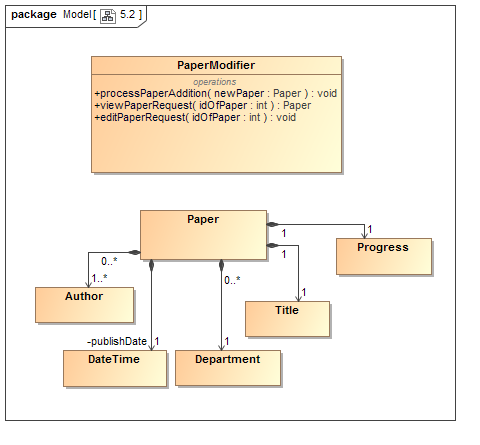
\includegraphics[width=\linewidth]{5.2.png}
					\caption{UML diagram for Request and Results Data Structure.}
				\end{figure}
				\clearpage
		\subsection{Required functionality}
			\begin{itemize}
				\item	Add a paper Use case: See figure 2
					\begin{figure}[!h]
						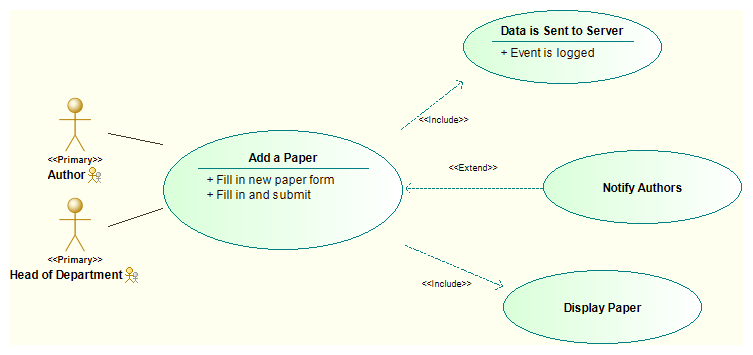
\includegraphics[width=\linewidth]{Add A Paper Use Case}
						\caption{Use case diagram for adding a paper}				
					\end{figure}
				\item   Edit a paper Use case: See figure 3
					\begin{figure}[!h]
						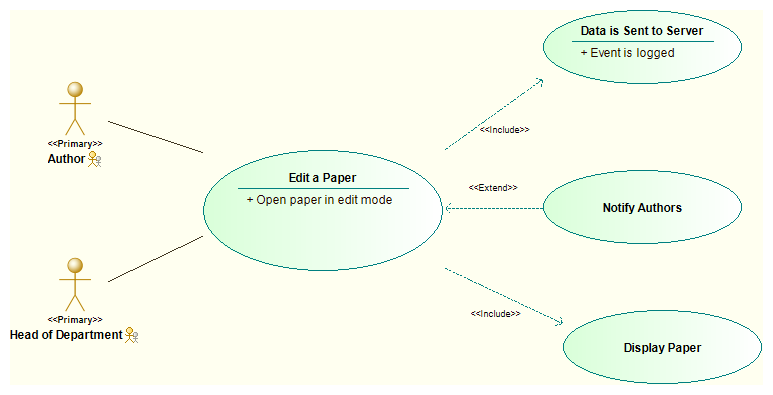
\includegraphics[width=\linewidth]{Edit a Paper Use Case}
						\caption{Use case diagram for editing a paper}				
					\end{figure}
				\item   View a paper Use case: See figure 4		
					\begin{figure}[!h]
						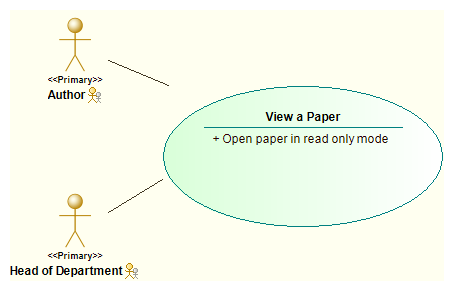
\includegraphics[width=\linewidth]{View a paper Use Case}
						\caption{Use case diagram for viewing a paper}
					\end{figure}									
			\end{itemize}
			\clearpage
		\subsection{Process specifications}
			\begin{itemize}
				\item Activity diagram to add a paper: See figure 5
					\begin{figure}[!h]
						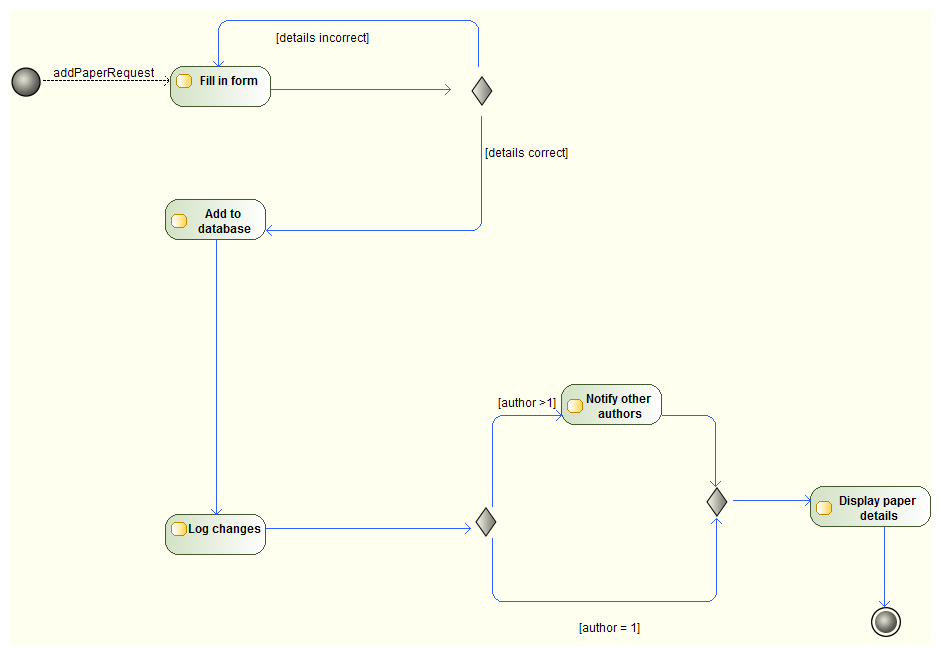
\includegraphics[width=\linewidth]{Activity diagram-Add a paper.png}
						\caption{Adding a paper to the database}
					\end{figure}
				\item Activity diagram to edit a paper: See figure 6
					\begin{figure}[!h]
						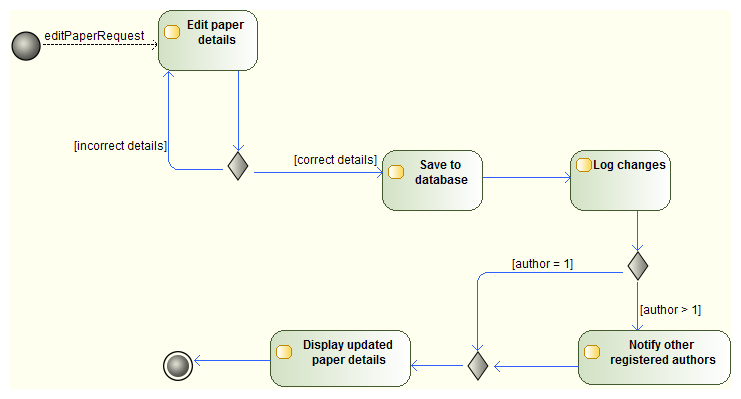
\includegraphics[width=\linewidth]{Activity diagram_Edit a paper.png}
						\caption{Editing a paper}
					\end{figure}
				\item Activity diagram to Login: See figure 7
						\begin{figure}[!h]
							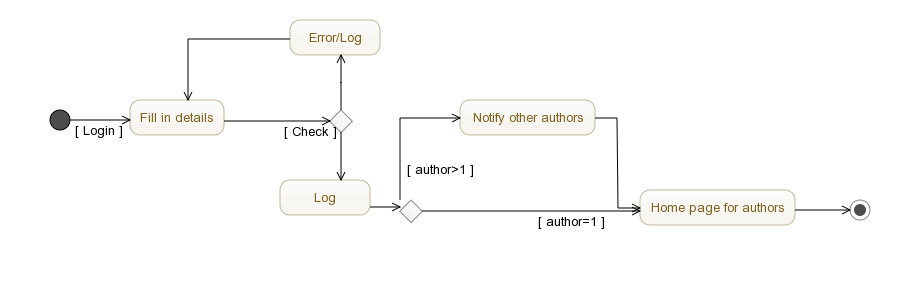
\includegraphics[width=\linewidth]{Activity.Login.jpg}
							\caption{Login to system}
						\end{figure}
				\item Activity diagram to Request document details: See figure 8
					\begin{figure}[!h]
						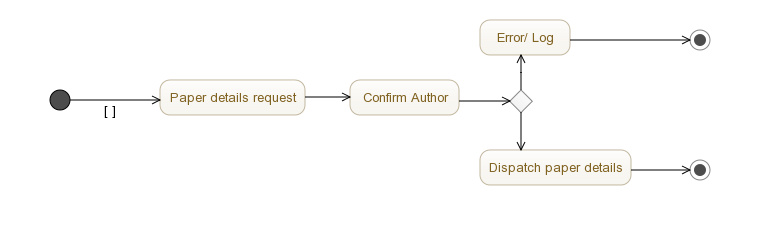
\includegraphics[width=\linewidth]{Pictures/Request.Paper.jpg}
						\caption{Request paper details}
					\end{figure}	
			\end{itemize}
			\clearpage
		\subsection{Domain Model}
			\begin{list}{$\bullet$}{\leftmargin=1.5cm \itemindent=0em}
				\item Domain Model of the system: See figure 9
					\begin{figure}[h!]
						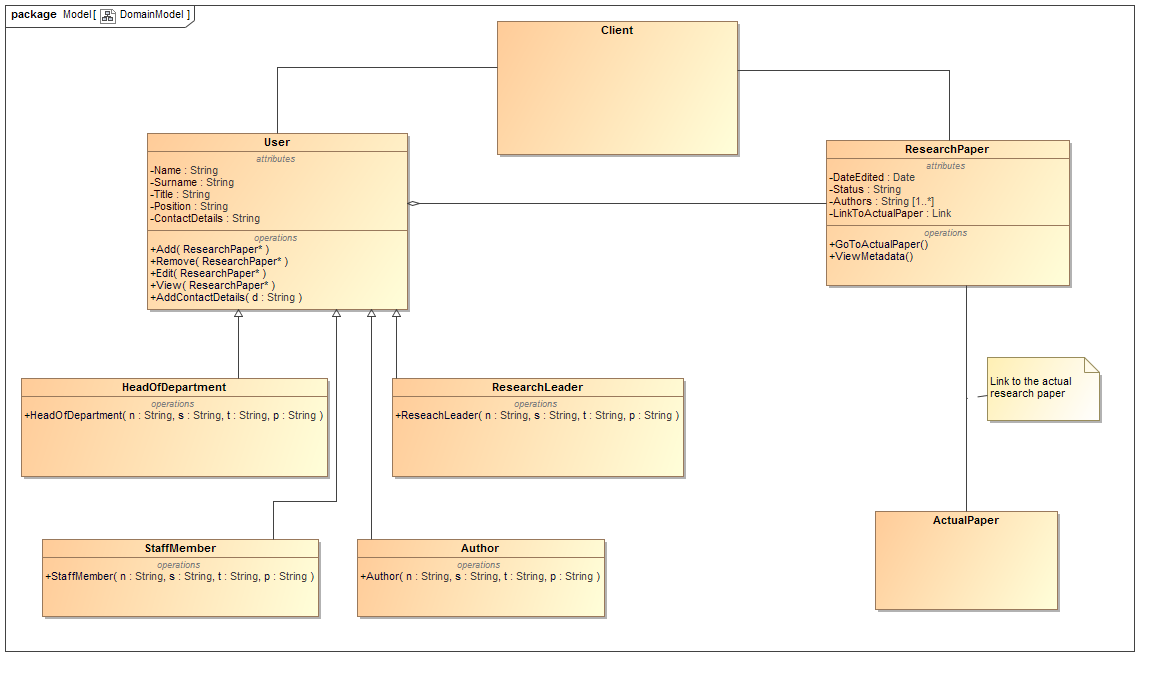
\includegraphics[width=\linewidth]{Pictures/5-5.png}
						\caption{Domain Model}
					\end{figure}
			\end{list}
			\clearpage
	\section{Software Architecture Documentation}
		\subsection{Architecture requirements}

			\subsubsection{Architectural scope}
			
				\paragraph\indent
				The architectural responsibilities that need to be handled by the software architecture are as follows:
				\begin{list}{$\bullet$}{\leftmargin=1.5cm \itemindent=0em}
					\item A main database that will store the papers that are added.
					\item A secondary database (separate from the first) that will act as the backup database where the partial and complete dumps will be stored.
					\item An infrastructure that will allow for notification to contributing authors that changes have been made to a paper they collaborated on, this infrastructure will also create a log of changes and who made them so that there is accountability.
					\item An infrastructure that will allow the users of the system to create and add papers to the database mentioned above as well as being able to edit and view them later.
					\item A mobile version of the above previously mentioned infrastructure must also exist. 
				\end{list}
			\subsubsection{Quality requirements}
				\paragraph\indent
				In order of importance our quality requirements are:
				\begin{list}{$\bullet$}{\leftmargin=1.5cm \itemindent=0em}
					\item \textbf{Reliability:} This is highly important as this might be the only place research could be backed up to, therefore, the system needs to be reliable. Reliability in this system is measured against the effectiveness of the backup measures in place as well as the system be available on demand. This will be achieved by an automatic partial dump backup occurring daily in the early hours of the morning and a full dump once every 3 days.
					\item \textbf{Security:} The system needs to be secure from anyone who does not (or should not) have permission to use, therefore, passwords will be secured using the SHA512 hashing algorithm.
					\item \textbf{Audibility:} This is measured in terms of is every change noted and logged somewhere. This will be done through means of recording, when a change is made, the system will log the change as well as the user name that submitted the change, therefore everyone will be held accountable.
					\item \textbf{Scalability:} There will not be a huge amount of users making use of the system but it is important that if need be every user can make use of the system concurrently. This will be achieved by implementing the system in such a way that it is multi-threaded. In terms of two users trying work on the same paper simultaneously, when a user tries to upload an edited version of the paper, if the version on the system differs from the original document then the user will be alerted that there is a synchronization error and he should update the local version of the document and add the changes. This will avoid data corruption.
					\item \textbf{Maintainability:} Measured against how effectively the system choses to relocate data due to age. When data has been on the system for a predetermined length of time, it will be moved from the main system and relocated to a different (most likely slower) database and if a user wishes to make use of it again it can be called from there.
				\end{list}
			
			\subsubsection{Integration and access channel requirements}
			
			\subsubsection{Architectural constraints}
			
		\subsection{Architectural patterns or styles}
		
		\subsection{Architectural tactics or strategies}
			\paragraph{Performance}\indent
			To better manage resource intensive tasks thread pooling will be used. There will be an object that receives all tasks and allocates them to a specified thread when a thread becomes available.
			
			\paragraph{Exception handling}\indent
			Exceptions should be dealt with as soon as and as best as possible, but since it cannot be afforded that the system crashes there should be some form of "last resort" that attempts to deal with unhandled exceptions in such a way that the system as a whole keep functioning.
			
			\paragraph{Passive Redundency}\indent
			There will be 2 databases that will both contain all the information. This will increase the reliability of the system by having a back up database that can take over at any point when the primary database fails. This will be transparent to the user.
			
			\paragraph{Transactions}\indent
			Changes to the database will be done in transactions that will allow any changes to be rolled back to s checkpoint should an error occur. This will cause atomicity in the system and increase reliability.
			
			\paragraph{Security}\indent
			Encryption to increase security https protocols will be used to transmit data and all private information (like passwords) will be hashed using the SHA512 hashing algorithm.
			
			\paragraph{Interatability}\indent
			In order to increase interatability a modular approach will be taken when implementing the system by using dependency injection as far as possile.
			
		\subsection{Use of reference architectures and frameworks}
			\paragraph\indent The frameworks listed here all reduce development time and cost of the system.
			\begin{itemize}
				\item Bootstrap for styling the Web interface of the system. Will be used for alignment of the elements ofthe web interface, any alignment for tables (if any) and responsive design so that the  web intergace can be viewed on mobile devices.
				\item AngularJS will be used for the front end of the website along with bootstrap by using UI Bootstrap. For example will be used for DOM manipulation and data-binding can be used to send data to the server. Most notable and obvious use is when a new user creates an account, angularJS will handle and send the data entred by the user to the server.
				\item PhoneGap (renamed to Apache Cordova, we will use PhoneGap in this document) will be used as a wrapper for the above website in mobile form. Meaning the web interface will be used and PhoneGap will create a hybrid Android app that communicates with the server and only acts as an interface to enter data.
				\item Ionic framework will be used together with AngularJS and PhoneGap and replace Bootstrap for the hybrid android app. ionic makes better and responsive apps when used with PhoneGap and requires angularJs. The reason it will replace Bootstrap for the mobile app is because Bootstrap and Ionic do not play well because of name conflicts.
				\item Spring framework will be mainly used for dependancy injection on the server side of the system. The MVC nature of Spring will also be of good use for the needs of the system. Spring is also some kind of wrapper for Java EE.
				\item Java EE can be seen as a reference architecture that supports scalability, MVC and dependancy injection. All are needed fo be implemented in the CS Research System.
			\end{itemize}
			
		\subsection{Access and integration channels}
		
		\subsection{Technologies}
			\paragraph\indent
			Technologies used will be MySQL for the database , it is very light weight and will have sufficient access control for the given product. The server will be a mix of PHP and Java, both will connect to MySQL , the Java will be the host for the android connection and the PHP will handle requests from the web interface. (Just a suggestion... Java is a bit better than php in some aspects, so I said that we use spring, that uses java. But we can use php for the report generation, by using the TCPDF php class - Charl)
	\section{Open Issues}	
		\paragraph\indent	
		There are currently no open issues.
\end{document}
